\begin{enumerate}[label=\thesection.\arabic*,ref=\thesection.\theenumi]
\numberwithin{equation}{enumi}
\numberwithin{figure}{enumi}
\numberwithin{table}{enumi}

	\item Find the coordinates of the focii, the vertices, the eccentricity and the length of the latus rectum of a hyperbola whose equation is given by $\frac{x^2}{16}-\frac{y^2}{9} = 1$. \\ 
		\solution
		\iffalse
\documentclass[12pt]{article}
\usepackage{graphicx}
\usepackage[none]{hyphenat}
\usepackage{graphicx}
\usepackage{listings}
\usepackage[english]{babel}
\usepackage{graphicx}
\usepackage{caption} 
\usepackage{booktabs}
\usepackage{array}
\usepackage{amssymb} % for \because
\usepackage{amsmath}   % for having text in math mode
\usepackage{extarrows} % for Row operations arrows
\usepackage{listings}
\lstset{
  frame=single,
  breaklines=true
}
\usepackage{hyperref}
  
%Following 2 lines were added to remove the blank page at the beginning
\usepackage{atbegshi}% http://ctan.org/pkg/atbegshi
\AtBeginDocument{\AtBeginShipoutNext{\AtBeginShipoutDiscard}}


%New macro definitions
\newcommand{\mydet}[1]{\ensuremath{\begin{vmatrix}#1\end{vmatrix}}}
\providecommand{\brak}[1]{\ensuremath{\left(#1\right)}}
\providecommand{\norm}[1]{\left\lVert#1\right\rVert}
\providecommand{\abs}[1]{\left\vert#1\right\vert}
\newcommand{\solution}{\noindent \textbf{Solution: }}
\newcommand{\myvec}[1]{\ensuremath{\begin{pmatrix}#1\end{pmatrix}}}
\let\vec\mathbf


\begin{document}

\begin{center}
\title{\textbf{Conic Sections - Hyperbola}}
\date{\vspace{-5ex}} %Not to print date automatically
\maketitle
\end{center}
\setcounter{page}{1}

\section{11$^{th}$ Maths - Chapter 11}
This is Problem-1 from Exercise 11.4
\begin{enumerate}
\solution 
From the given equation of hyperbola, we can get values of
\begin{align}
    a = 4 \\
    b = 3
\end{align}
The given equation of the hyperbola can be rearranged as
\begin{align}
    \label{eq:11/11/4/1hyperEq1}
    9x^2 - 16y^2-144 = 0 
\end{align}
\fi
The given equation can be equated to the generic equation of conic sections
\iffalse
\begin{align}
	\label{eq:11/11/4/1hyperEq2}
	g\brak{\vec{x}} = \vec{x}^T\vec{V}\vec{x} + 2\vec{u}^T\vec{x} + f = 0 
\end{align}
Comparing coefficients of both equations \eqref{eq:11/11/4/1hyperEq1} and \eqref{eq:11/11/4/1hyperEq2} 
\fi
a
\begin{align}
	\label{eq:11/11/4/1eqV}
	\vec{V} &= \myvec{ 9 & 0 \\ 0 & -16} \\
	\label{eq:11/11/4/1eqU}
	\vec{u} &=  0 \\
	\label{eq:11/11/4/1eqF}
	f &= -144 
\end{align}
From equation \eqref{eq:11/11/4/1eqV}, since $\vec{V}$ is already diagonalized, the Eigen values $\lambda_1$ and $\lambda_2$ are given as 
\begin{align}
	\label{eq:11/11/4/1eqEigen1}
	\lambda_1 &= 9 \\
	\label{eq:11/11/4/1eqEigen2}
	\lambda_2 &= -16 
\end{align}
\begin{enumerate}
\item The eccentricity of the hyperbola is given as  
\begin{align}
	e &= \sqrt{1-\frac{\lambda_1}{\lambda_2}} \\
	  &= \sqrt{1-\frac{9}{-16}} \\
          &= \frac{5}{4}
\end{align}
\item For the standard hyperbola, the coordinates of Focii are given as: 
\begin{align}
	\label{eq:11/11/4/1eqFocus}
	\vec{F} &= \pm \frac{\brak{\frac{1}{e\sqrt{1-e^2}}}\brak{e^2}\sqrt{\frac{\lambda_2}{f_0}}}{\frac{\lambda_2}{f_0}}\vec{e1} 
\end{align}
where
\begin{align}
	f_0 &= -f \\
	\eqref{eq:11/11/4/1eqFocus} \implies &=  \pm \frac{\brak{\frac{1}{\frac{5}{4}\sqrt{1-\frac{25}{16}}}}\brak{\frac{25}{16}}\sqrt{\frac{-16}{144}}\vec{e_1}}{\frac{-16}{144}} \\
	&= \pm \myvec{5 \\ 0}
\end{align}
\item The vertices of the hyperbola are given by 
\begin{align}
	& \pm\myvec{ a \\ 0} \\
	&= \pm\myvec{4 \\ 0}
\end{align}
\item The length of the latus rectum is given as 
\begin{align}
	\label{eq:11/11/4/1eqLatRectLen}
	& 2\frac{\sqrt{\abs{f_0\lambda_1}}}{\lambda_2} \\
	&= 2\frac{\sqrt{\abs{144\brak{9}}}}{-16} \\
	&= \frac{9}{2}
\end{align}
as length can't be negative. 
The relevant diagram is shown in Figure \ref{fig:11/11/4/1Fig1}
\begin{figure}[!h]
	\begin{center}
		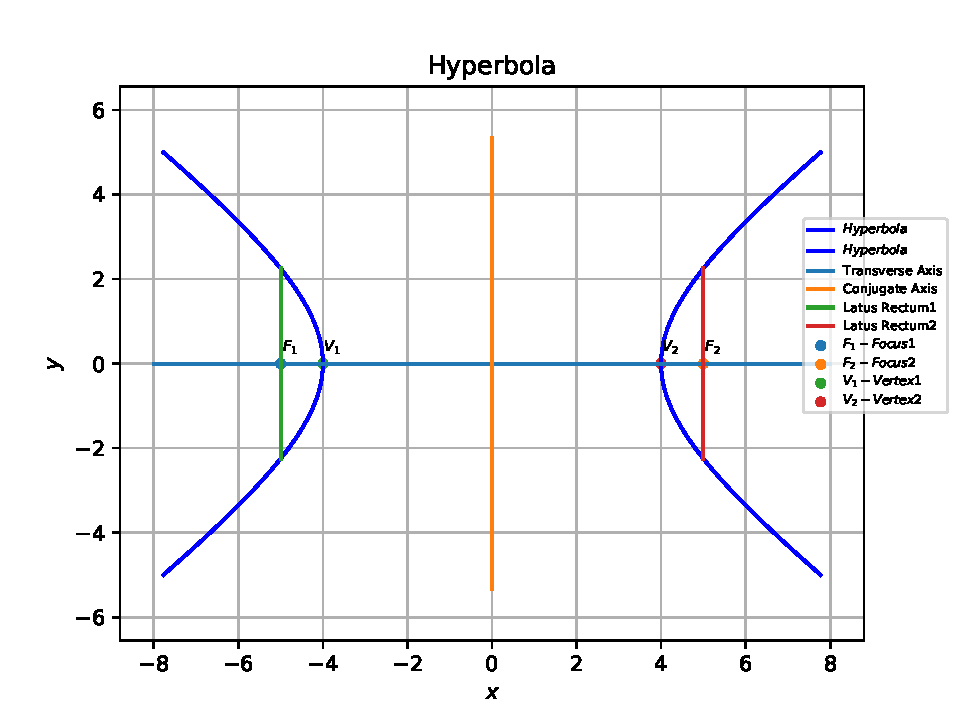
\includegraphics[width=\columnwidth]{chapters/11/11/4/1/figs/problem1.pdf}
	\end{center}
\caption{}
\label{fig:11/11/4/1Fig1}
\end{figure}
\end{enumerate}

	\item Find the coordinates of the focii, the vertices, the eccentricity and the length of the latus rectum of a hyperbola whose equation is given by $\frac{y^2}{9}-\frac{x^2}{27}=1$.
		\\
		\solution
		\\
		\iffalse
\documentclass[12pt]{article}
\usepackage{graphicx}
\usepackage{amsmath}
\usepackage{mathtools}
\usepackage{gensymb}

\newcommand{\mydet}[1]{\ensuremath{\begin{vmatrix}#1\end{vmatrix}}}
\providecommand{\brak}[1]{\ensuremath{\left(#1\right)}}
\providecommand{\norm}[1]{\left\lVert#1\right\rVert}
\providecommand{\abs}[1]{\left\vert#1\right\vert}
\newcommand{\solution}{\noindent \textbf{Solution: }}
\newcommand{\myvec}[1]{\ensuremath{\begin{pmatrix}#1\end{pmatrix}}}
\let\vec\mathbf

\begin{document}
\begin{center}
\textbf\large{CONIC SECTIONS}

\end{center}
\section*{Excercise 11.4}
\solution
\fi
The equation of the hyperbola can be rearranged as
\begin{align}
	\label{eq:chapters/11/11/4/2/eq1}
	-x^2 + 3y^2 -27 = 0
\end{align}
The above equation can be equaded to the generic equation of conic sections
\begin{align}
	\label{eq:chapters/11/11/4/2/eq2}
	g\brak{\vec{x}}=\vec{x}^\top \vec{V} \vec{x} + 2\vec{u}^\top \vec{x} + f = 0
\end{align}
Comparing coefficients of both equations \eqref{eq:chapters/11/11/4/2/eq1} and \eqref{eq:chapters/11/11/4/2/eq2}
\begin{align}
	\label{eq:chapters/11/11/4/2/eq3}
	\vec{V} &= \myvec{-1&0\\0&3}\\
	\vec{u} &= \vec{0}\\
	f &= -27
\end{align}
From equation \eqref{eq:chapters/11/11/4/2/eq3}, since $\vec{V}$ is already diagonalized, the eigen values $\lambda_1 \text{ and } \lambda_2$ are given as
\begin{align}
	\lambda_1 &= -1\\
	\lambda_2 &= 3
\end{align}
\begin{enumerate}
\item The eccentricity of the hyperbola is given as
\begin{align}
	e &= \sqrt{1 - \frac{\lambda_2}{\lambda_1}} = \sqrt{1+\frac{3}{1}}\\
	  &= 2
\end{align}
\item For the standard hyperbola, the coordinates of Focii are given as
\begin{align}
	\label{eq:chapters/11/11/4/2/eq4}
	\vec{F} = \pm \frac{\brak{\frac{1}{e\sqrt{1-e^2}}}\brak{e^2}\sqrt{\frac{\lambda_1}{f_0}}}{\frac{\lambda_1}{f_0}} \vec{e}_2
\end{align}
where
\begin{align}
	f_0 &= -f\\
	\eqref{eq:chapters/11/11/4/2/eq4} \implies &= \pm \frac{\brak{\frac{1}{2\sqrt{1-4}}}\brak{4}\sqrt{\frac{-1}{27}}}{\frac{-1}{27}} \vec{e}_2\\
	&= \pm \myvec{0\\6}
\end{align}
\item The vertices of the hyperbola are given by
\begin{align}
	\pm \myvec{0\\\sqrt{\abs{\frac{f_0}{\lambda_2}}}}= \pm \myvec{0\\3}
\end{align}
\item The length of latus rectum is given as
\begin{align}
	2\frac{\sqrt{\abs{f_0 \lambda_2}}}{\lambda_1} &= 2\frac{\sqrt{\abs{27\brak{3}}}}{-1}\\
	&= 18
\end{align}
as length cannot be negative.
\end{enumerate}
See Fig. \ref{fig:chapters/11/11/4/2/Fig1}
\begin{figure}[!h]
	\begin{center} 
	    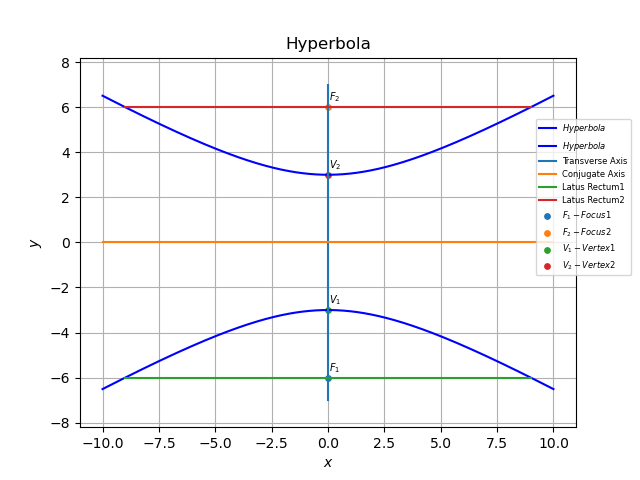
\includegraphics[width=\columnwidth]{chapters/11/11/4/2/figs/hyperbola}
	\end{center}
\caption{}
\label{fig:chapters/11/11/4/2/Fig1}
\end{figure}




	\item Find the coordinates of the foci and the vertices, the eccentricity and the length of the latus rectum of the hyperbolas, whose equation is given by $5{y^2}-9{x^2}=36$.
		\\
		\solution
		\\
		\iffalse
\documentclass[journal,12pt,twocolumn]{IEEEtran}
\usepackage{setspace}
\usepackage{gensymb}
\usepackage{xcolor}
\usepackage{caption}
\singlespacing
\usepackage{siunitx}
\usepackage[cmex10]{amsmath}
\usepackage{mathtools}
\usepackage{hyperref}
\usepackage{amsthm}
\usepackage{mathrsfs}
\usepackage{txfonts}
\usepackage{stfloats}
\usepackage{cite}
\usepackage{cases}
\usepackage{subfig}
\usepackage{longtable}
\usepackage{multirow}
\usepackage{enumitem}
\usepackage{bm}
\usepackage{mathtools}
\usepackage{listings}
\usepackage{tikz}
\usetikzlibrary{shapes,arrows,positioning}
\usepackage{circuitikz}
\renewcommand{\vec}[1]{\boldsymbol{\mathbf{#1}}}
\DeclareMathOperator*{\Res}{Res}
\renewcommand\thesection{\arabic{section}}
\renewcommand\thesubsection{\thesection.\arabic{subsection}}
\renewcommand\thesubsubsection{\thesubsection.\arabic{subsubsection}}

\renewcommand\thesectiondis{\arabic{section}}
\renewcommand\thesubsectiondis{\thesectiondis.\arabic{subsection}}
\renewcommand\thesubsubsectiondis{\thesubsectiondis.\arabic{subsubsection}}
\hyphenation{op-tical net-works semi-conduc-tor}

\lstset{
language=Python,
frame=single, 
breaklines=true,
columns=fullflexible
}
\begin{document}
\theoremstyle{definition}
\newtheorem{theorem}{Theorem}[section]
\newtheorem{problem}{Problem}
\newtheorem{proposition}{Proposition}[section]
\newtheorem{lemma}{Lemma}[section]
\newtheorem{corollary}[theorem]{Corollary}
\newtheorem{example}{Example}[section]
\newtheorem{definition}{Definition}[section]
\newcommand{\BEQA}{\begin{eqnarray}}
        \newcommand{\EEQA}{\end{eqnarray}}
\newcommand{\define}{\stackrel{\triangle}{=}}
\newcommand{\myvec}[1]{\ensuremath{\begin{pmatrix}#1\end{pmatrix}}}
\newcommand{\mydet}[1]{\ensuremath{\begin{vmatrix}#1\end{vmatrix}}}
\bibliographystyle{IEEEtran}
\providecommand{\nCr}[2]{\,^{#1}C_{#2}} % nCr
\providecommand{\nPr}[2]{\,^{#1}P_{#2}} % nPr
\providecommand{\mbf}{\mathbf}
\providecommand{\pr}[1]{\ensuremath{\Pr\left(#1\right)}}
\providecommand{\qfunc}[1]{\ensuremath{Q\left(#1\right)}}
\providecommand{\sbrak}[1]{\ensuremath{{}\left[#1\right]}}
\providecommand{\lsbrak}[1]{\ensuremath{{}\left[#1\right.}}
\providecommand{\rsbrak}[1]{\ensuremath{{}\left.#1\right]}}
\providecommand{\brak}[1]{\ensuremath{\left(#1\right)}}
\providecommand{\lbrak}[1]{\ensuremath{\left(#1\right.}}
\providecommand{\rbrak}[1]{\ensuremath{\left.#1\right)}}
\providecommand{\cbrak}[1]{\ensuremath{\left\{#1\right\}}}
\providecommand{\lcbrak}[1]{\ensuremath{\left\{#1\right.}}
\providecommand{\rcbrak}[1]{\ensuremath{\left.#1\right\}}}
\theoremstyle{remark}
\newtheorem{rem}{Remark}
\newcommand{\sgn}{\mathop{\mathrm{sgn}}}
\newcommand{\rect}{\mathop{\mathrm{rect}}}
\newcommand{\sinc}{\mathop{\mathrm{sinc}}}
\providecommand{\abs}[1]{\left\vert#1\right\vert}
\providecommand{\res}[1]{\Res\displaylimits_{#1}}
\providecommand{\norm}[1]{\lVert#1\rVert}
\providecommand{\mtx}[1]{\mathbf{#1}}
\providecommand{\mean}[1]{E\left[ #1 \right]}
\providecommand{\fourier}{\overset{\mathcal{F}}{ \rightleftharpoons}}
\providecommand{\ztrans}{\overset{\mathcal{Z}}{ \rightleftharpoons}}
\providecommand{\system}[1]{\overset{\mathcal{#1}}{ \longleftrightarrow}}
\newcommand{\solution}{\noindent \textbf{Solution: }}
\providecommand{\dec}[2]{\ensuremath{\overset{#1}{\underset{#2}{\gtrless}}}}
\let\StandardTheFigure\thefigure
\def\putbox#1#2#3{\makebox[0in][l]{\makebox[#1][l]{}\raisebox{\baselineskip}[0in][0in]{\raisebox{#2}[0in][0in]{#3}}}}
\def\rightbox#1{\makebox[0in][r]{#1}}
\def\centbox#1{\makebox[0in]{#1}}
\def\topbox#1{\raisebox{-\baselineskip}[0in][0in]{#1}}
\def\midbox#1{\raisebox{-0.5\baselineskip}[0in][0in]{#1}}

\vspace{3cm}
\title{11.11.4.5}
\author{Lokesh Surana}
\maketitle
\section*{Class 11, Chapter 11, Exercise 4.5}
\fi
The equation of the hyperbola can be rearranged as
\begin{align}
	\label{eq:chapters/11/11/4/5/1}
	-x^2 + \frac{5}{9}y^2 -4 = 0
\end{align}
The above equation can be equaded to the generic equation of conic sections
\begin{align}
	\label{eq:chapters/11/11/4/5/2}
	g\brak{\vec{x}}=\vec{x}^\top \vec{V} \vec{x} + 2\vec{u}^\top \vec{x} + f = 0
\end{align}
Comparing coefficients of both equations \eqref{eq:chapters/11/11/4/5/1} and \eqref{eq:chapters/11/11/4/5/2}
\begin{align}
	\label{3}
	\vec{V} &= \myvec{-1&0\\0&\frac{5}{9}}\\
	\vec{u} &= \vec{0}\\
	f &= -4
\end{align}

From equation \eqref{3}, since $\vec{V}$ is already diagonalized, the eigen values $\lambda_1 \text{ and } \lambda_2$ are given as
\begin{align}
	\lambda_1 &= -1\\
	\lambda_2 &= \frac{5}{9}
\end{align}
\begin{enumerate}
\item The eccentricity of the hyperbola is given as
\begin{align}
	e &= \sqrt{1 - \frac{\lambda_2}{\lambda_1}} = \sqrt{1+\frac{5}{9}}\\
	  &= \frac{\sqrt{14}}{3}
\end{align}
\item For the standard hyperbola, the coordinates of Focii are given as
\begin{align}
	\label{eq:chapters/11/11/4/5/4}
	\vec{F} = \pm \frac{\brak{\frac{1}{e\sqrt{1-e^2}}}\brak{e^2}\sqrt{\frac{\lambda_1}{f_0}}}{\frac{\lambda_1}{f_0}} \vec{e}_2
\end{align}
where
\begin{align}
	f_0 &= -f\\
	\eqref{eq:chapters/11/11/4/5/4} \implies &= \pm \frac{\brak{\frac{1}{\frac{\sqrt{14}}{3}\sqrt{1-\frac{14}{9}}}}\brak{\frac{14}{9}}\sqrt{\frac{-1}{4}}}{\frac{-1}{4}} \vec{e}_2\\
	&= \pm \myvec{0\\\frac{6}{2\sqrt{\frac{14}{5}}}}
\end{align}
\item The vertices of the hyperbola are given by
\begin{align}
	\pm \myvec{0\\\sqrt{\abs{\frac{f_0}{\lambda_2}}}}= \pm \myvec{0\\\frac{6}{\sqrt{5}}}
\end{align}
\item The length of latus rectum is given as
\begin{align}
	2\frac{\sqrt{\abs{f_0 \lambda_2}}}{\lambda_1} &= 2\frac{\sqrt{\abs{14\brak{\frac{5}{9}}}}}{-1}\\
	&= 4\frac{\sqrt{5}}{3}
\end{align}
as length cannot be negative.
\end{enumerate}

\begin{figure}[!h]
	\begin{center} 
	    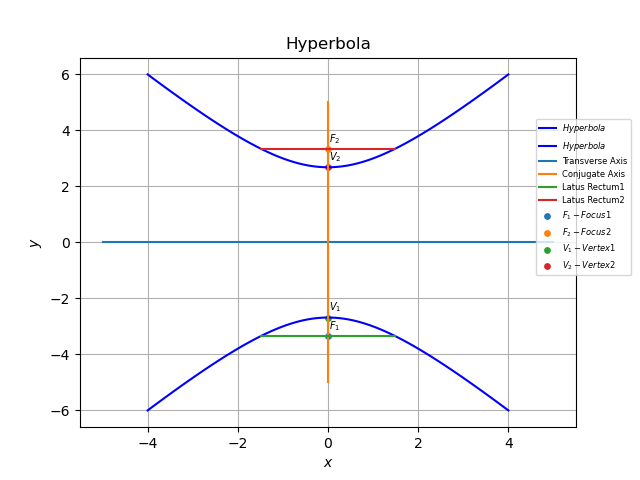
\includegraphics[width=\columnwidth]{chapters/11/11/4/5/figs/hyperbola.png}
	\end{center}
\caption{}
\label{fig:chapters/11/11/4/5/1}
\end{figure}


	\item Find the equation of the hyperbola whose foci is $\brak{0,\pm 8}$ and vertices $\brak{0,\pm 5}$.
\\
\solution
\item Find the equations of hyperbola having Vertices $\myvec{0\\\pm 3}$ and Foci $\myvec{0\\\pm5}$
	\\
\solution
		\iffalse
\documentclass[journal,12pt,twocolumn]{IEEEtran}
%
\usepackage{setspace}
\usepackage{gensymb}
%\doublespacing
\singlespacing

%\usepackage{graphicx}
%\usepackage{amssymb}
%\usepackage{relsize}
\usepackage[cmex10]{amsmath}
%\usepackage{amsthm}
%\interdisplaylinepenalty=2500
%\savesymbol{iint}
%\usepackage{txfonts}
%\restoresymbol{TXF}{iint}
%\usepackage{wasysym}
\usepackage{amsthm}
%\usepackage{iithtlc}
\usepackage{mathrsfs}
\usepackage{txfonts}
\usepackage{stfloats}
\usepackage{bm}
\usepackage{cite}
\usepackage{cases}
\usepackage{subfig}
%\usepackage{xtab}
\usepackage{longtable}
\usepackage{multirow}
%\usepackage{algorithm}
%\usepackage{algpseudocode}
\usepackage{enumitem}
\usepackage{mathtools}
\usepackage{steinmetz}
\usepackage{tikz}
\usepackage{circuitikz}
\usepackage{verbatim}
\usepackage{tfrupee}
\usepackage[breaklinks=true]{hyperref}
%\usepackage{stmaryrd}
\usepackage{tkz-euclide} % loads  TikZ and tkz-base
%\usetkzobj{all}
\usetikzlibrary{calc,math}
\usepackage{listings}
    \usepackage{color}                                            %%
    \usepackage{array}                                            %%
    \usepackage{longtable}                                        %%
    \usepackage{calc}                                             %%
    \usepackage{multirow}                                         %%
    \usepackage{hhline}                                           %%
    \usepackage{ifthen}                                           %%
  %optionally (for landscape tables embedded in another document): %%
    \usepackage{lscape}     
\usepackage{multicol}
\usepackage{chngcntr}
%\usepackage{enumerate}

%\usepackage{wasysym}
%\newcounter{MYtempeqncnt}
\DeclareMathOperator*{\Res}{Res}
%\renewcommand{\baselinestretch}{2}
\renewcommand\thesection{\arabic{section}}
\renewcommand\thesubsection{\thesection.\arabic{subsection}}
\renewcommand\thesubsubsection{\thesubsection.\arabic{subsubsection}}

\renewcommand\thesectiondis{\arabic{section}}
\renewcommand\thesubsectiondis{\thesectiondis.\arabic{subsection}}
\renewcommand\thesubsubsectiondis{\thesubsectiondis.\arabic{subsubsection}}

% correct bad hyphenation here
\hyphenation{op-tical net-works semi-conduc-tor}
\def\inputGnumericTable{}                                 %%

\lstset{
%language=C,
frame=single, 
breaklines=true,
columns=fullflexible
}
%\lstset{
%language=tex,
%frame=single, 
%breaklines=true
%}

\begin{document}
%


\newtheorem{theorem}{Theorem}[section]
\newtheorem{problem}{Problem}
\newtheorem{proposition}{Proposition}[section]
\newtheorem{lemma}{Lemma}[section]
\newtheorem{corollary}[theorem]{Corollary}
\newtheorem{example}{Example}[section]
\newtheorem{definition}[problem]{Definition}
%\newtheorem{thm}{Theorem}[section] 
%\newtheorem{defn}[thm]{Definition}
%\newtheorem{algorithm}{Algorithm}[section]
%\newtheorem{cor}{Corollary}
\newcommand{\BEQA}{\begin{eqnarray}}
\newcommand{\EEQA}{\end{eqnarray}}
\newcommand{\define}{\stackrel{\triangle}{=}}

\bibliographystyle{IEEEtran}
%\bibliographystyle{ieeetr}


\providecommand{\mbf}{\mathbf}
\providecommand{\pr}[1]{\ensuremath{\Pr\left(#1\right)}}
\providecommand{\qfunc}[1]{\ensuremath{Q\left(#1\right)}}
\providecommand{\sbrak}[1]{\ensuremath{{}\left[#1\right]}}
\providecommand{\lsbrak}[1]{\ensuremath{{}\left[#1\right.}}
\providecommand{\rsbrak}[1]{\ensuremath{{}\left.#1\right]}}
\providecommand{\brak}[1]{\ensuremath{\left(#1\right)}}
\providecommand{\lbrak}[1]{\ensuremath{\left(#1\right.}}
\providecommand{\rbrak}[1]{\ensuremath{\left.#1\right)}}
\providecommand{\cbrak}[1]{\ensuremath{\left\{#1\right\}}}
\providecommand{\lcbrak}[1]{\ensuremath{\left\{#1\right.}}
\providecommand{\rcbrak}[1]{\ensuremath{\left.#1\right\}}}
\theoremstyle{remark}
\newtheorem{rem}{Remark}
\newcommand{\sgn}{\mathop{\mathrm{sgn}}}
\providecommand{\abs}[1]{\left\vert#1\right\vert}
\providecommand{\res}[1]{\Res\displaylimits_{#1}} 
\providecommand{\norm}[1]{\left\lVert#1\right\rVert}
%\providecommand{\norm}[1]{\lVert#1\rVert}
\providecommand{\mtx}[1]{\mathbf{#1}}
\providecommand{\mean}[1]{E\left[ #1 \right]}
\providecommand{\fourier}{\overset{\mathcal{F}}{ \rightleftharpoons}}
%\providecommand{\hilbert}{\overset{\mathcal{H}}{ \rightleftharpoons}}
\providecommand{\system}{\overset{\mathcal{H}}{ \longleftrightarrow}}
	%\newcommand{\solution}[2]{\textbf{Solution:}{#1}}
\newcommand{\solution}{\noindent \textbf{Solution: }}
\newcommand{\cosec}{\,\text{cosec}\,}
\providecommand{\dec}[2]{\ensuremath{\overset{#1}{\underset{#2}{\gtrless}}}}
\newcommand{\myvec}[1]{\ensuremath{\begin{pmatrix}#1\end{pmatrix}}}
\newcommand{\mydet}[1]{\ensuremath{\begin{vmatrix}#1\end{vmatrix}}}
%\numberwithin{equation}{section}
\numberwithin{equation}{subsection}
%\numberwithin{problem}{section}
%\numberwithin{definition}{section}
\makeatletter
\@addtoreset{figure}{problem}
\makeatother

\let\StandardTheFigure\thefigure
\let\vec\mathbf
%\renewcommand{\thefigure}{\theproblem.\arabic{figure}}
\renewcommand{\thefigure}{\theproblem}
%\setlist[enumerate,1]{before=\renewcommand\theequation{\theenumi.\arabic{equation}}
%\counterwithin{equation}{enumi}


%\renewcommand{\theequation}{\arabic{subsection}.\arabic{equation}}

\def\putbox#1#2#3{\makebox[0in][l]{\makebox[#1][l]{}\raisebox{\baselineskip}[0in][0in]{\raisebox{#2}[0in][0in]{#3}}}}
     \def\rightbox#1{\makebox[0in][r]{#1}}
     \def\centbox#1{\makebox[0in]{#1}}
     \def\topbox#1{\raisebox{-\baselineskip}[0in][0in]{#1}}
     \def\midbox#1{\raisebox{-0.5\baselineskip}[0in][0in]{#1}}

\vspace{3cm}


\title{Que: 11.11.4.9}
\author{Nikam Pratik Balasaheb (EE21BTECH11037)}





% make the title area
\maketitle

\newpage

%\tableofcontents

\bigskip

\renewcommand{\thefigure}{\theenumi}
\renewcommand{\thetable}{\theenumi}
%\renewcommand{\theequation}{\theenumi}

\section{Problem}

\section{Solution}
\fi

\begin{enumerate}

	\item Transverse axis:
Line joining two foci
\begin{align}
	\vec{m} &= \vec{F}_1 - \vec{F}_2\\
	&= \myvec{0 \\ 10}\\
	\myvec{1&0}\brak{\vec{x} -\vec{F}_1} &= 0\\
	\myvec{1& 0}\vec{x} &= 0
\end{align}

\item Center of hyperbola, $\vec{O}$ is given by:
\begin{align}
	\vec{O} &= \frac{\vec{F}_1 + \vec{F}_2}{2}\\
	\vec{O} &= \myvec{0\\0}
\end{align}

\item Normal vector of directrix
	\begin{align}
		\vec{n} &= \text{direction vector of transverse axis}\\
			&= \myvec{0 \\1}
	\end{align}
%
\begin{align}
	\vec{V} &= \norm{\vec{n}}^2\vec{I} - e^2\vec{n}\vec{n}^{\top}\\
		&= \myvec{1 & 0 \\ 0 & 1} - e^2\myvec{ 0 & 0 \\ 0 & 1}\\
		&= \myvec{1 &0\\ 0 & 1-e^2}
\end{align}
%
\begin{align}
	\vec{u} &= ce^2\vec{n} -\norm{\vec{n}}^2\vec{F}\\
		&= \myvec{0\\ ce^2 - 5}
\end{align}
%
\begin{align}
	f &= \norm{\vec{n}}^2\norm{\vec{F}}^2 - c^2e^2\\
	  &= 25 - c^2 e^2
\end{align}
%
Equation of the hyperbola
\begin{align}
	\vec{x}^{\top}\vec{V}\vec{x} +2\vec{u}^{\top}\vec{x}+f &= 0
\end{align}
%
Vertex lies on this curve,
\begin{align}
	\vec{v_1}^{\top}\vec{V}\vec{v_1} +2\vec{u}^{\top}\vec{v_1}+f &= 0\\
	9\brak{1-e^2} + 6 \brak{ce^2 -5} - c^2e^2 +25 &= 0\\
	4 -9e^2 +6ce^2 -c^2e^2 &= 0 \label{eq:chapters/11/11/4/9/1}
\end{align}
Also, the center is given by,
\begin{align}
	\vec{O} &= - \vec{V}^{-1} \vec{u}\\
	\myvec{0\\0} &= \myvec{0\\ \frac{ce^2-5}{1-e^2}}\\
	ce^2 &= 5
	\label{eq:chapters/11/11/4/9/2}
\end{align}
%
Solving \eqref{eq:chapters/11/11/4/9/1} and \eqref{eq:chapters/11/11/4/9/2},
\begin{align}
	c &= \frac{9}{5} \\
	e &= \frac{5}{3}
\end{align}
%
\begin{align}
	\vec{V} &= \myvec{1&0\\0& -\frac{16}{9}} \\
	\vec{u} &= \myvec{0\\0}\\
	f &= 16
\end{align}
%
Equation of the Hyperbola,
\begin{align}
	\vec{x}^{\top} \myvec{1&0\\ 0 & -\frac{16}{9}} \vec{x} +16 =0
\end{align}
%
\begin{table}[h!]
	\begin{center}
	%%%%%%%%%%%%%%%%%%%%%%%%%%%%%%%%%%%%%%%%%%%%%%%%%%%%%%%%%%%%%%%%%%%%%%
%%                                                                  %%
%%  This is a LaTeX2e table fragment exported from Gnumeric.        %%
%%                                                                  %%
%%%%%%%%%%%%%%%%%%%%%%%%%%%%%%%%%%%%%%%%%%%%%%%%%%%%%%%%%%%%%%%%%%%%%%

\begin{tabular}[]{|c|c|c|}
\hline
Parameter & Value & Description \\ \hline
$\vec{F}_1$	& $\myvec{0\\5}$ & Focus\\ \hline
$\vec{F}_2$	& $\myvec{0\\-5}$ & Focus\\ \hline
$\vec{v}_1$	& $\myvec{0\\3}$ & Vertex \\ \hline
$\vec{v}_2$ 	& $\myvec{0\\-3}$ & Vertex\\ \hline
\end{tabular}

\end{center}
\caption{}
\label{tab:chapters/11/11/4/9/}
\end{table}
%
\begin{figure}[h!]
  \centering
    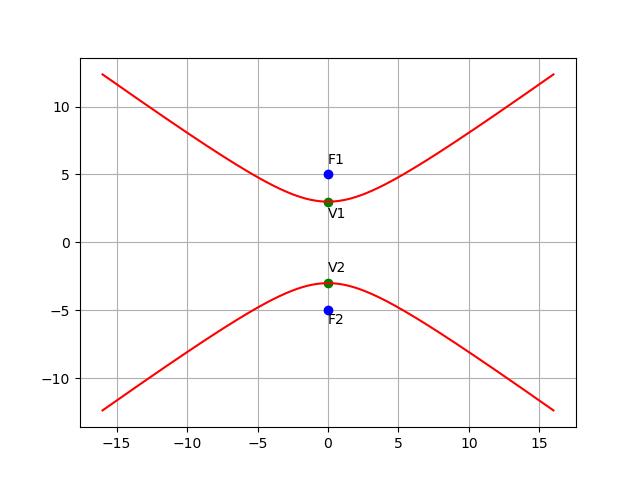
\includegraphics[width=\columnwidth]{chapters/11/11/4/9/figs/Figure_1.png}
    \caption{Figure 1}
    \label{fig:chapters/11/11/4/9/}
\end{figure}
%
\end{enumerate}




	\iffalse
\documentclass[12pt]{article}
\usepackage{graphicx}
\usepackage{amsmath}
\usepackage{mathtools}
\usepackage{gensymb}

\newcommand{\mydet}[1]{\ensuremath{\begin{vmatrix}#1\end{vmatrix}}}
\providecommand{\brak}[1]{\ensuremath{\left(#1\right)}}
\providecommand{\norm}[1]{\left\lVert#1\right\rVert}
\providecommand{\abs}[1]{\left\vert#1\right\vert}
\newcommand{\solution}{\noindent \textbf{Solution: }}
\newcommand{\myvec}[1]{\ensuremath{\begin{pmatrix}#1\end{pmatrix}}}
\let\vec\mathbf

\begin{document}
\begin{center}
\textbf\large{CONIC SECTIONS}

\end{center}
\section*{Excercise 11.4}
\fi
Given
\begin{align}
	\vec{F} = \myvec{0\\\pm 8}, \vec{V} = \myvec{0\\\pm 5} 
\end{align}
\begin{enumerate}
\item We know the vertex is given as
\begin{align}
	\vec{V} = \pm\myvec{0\\\sqrt{\frac{f_0}{\lambda_2}}} = \pm\myvec{0\\5}\\
	\label{eq:chapters/11/11/4/8/eq1}
	\implies f_0 = 25\lambda_2
\end{align}
\item We know the Focii is given as
\begin{align}
	\vec{F} &= \pm \frac{\brak{\frac{1}{e\sqrt{1-e^2}}}\brak{e^2}\sqrt{\frac{\lambda_1}{f_0}}}{\frac{\lambda_1}{f_0}}\vec{e}_2\\
	        &= \frac{\frac{e}{\sqrt{1-e^2}}}{\sqrt{\frac{\lambda_1}{f_0}}}\vec{e}_2
\end{align}
Substituting \eqref{eq:chapters/11/11/4/8/eq1} we get
\begin{align}
	\vec{F} &= 5e\vec{e}_2\\
	\myvec{0\\8} &= 5e\vec{e}_2\\
	\implies e &= \frac{8}{5}
\end{align}
\item Now we know the eccentricity is given as
\begin{align}
	e = \sqrt{1-\frac{\lambda_2}{\lambda_1}}\\
	\label{eq:chapters/11/11/4/8/eq2}
	\implies \frac{\lambda_2}{\lambda_1} = -\frac{39}{25}
\end{align}
\item Now we know from the standard equation
\begin{align}
	\label{eq:chapters/11/11/4/8/eq3}
	f = \norm{\vec{n}}^2 \norm{\vec{F}}^2 - c^2 e^2
\end{align}
Calculating $\vec{n} \text{ and } c$
\begin{align}
	\vec{n} &= \sqrt{\frac{\lambda_1}{f_0}}\vec{e}_2 = \frac{1}{5}\sqrt{\frac{\lambda_1}{\lambda_2}}\vec{e}_2\\
	        &= \frac{1}{\sqrt{-39}}\vec{e}_2\\
	c &= \frac{1}{e\sqrt{1-e^2}} = \frac{25}{8\sqrt{-39}}	
\end{align}
Now
\begin{align}
	\norm{\vec{n}}^2 &= -\frac{1}{39}\\
	\norm{\vec{F}}^2 &= 64
\end{align}
Substituting all the values in \eqref{eq:chapters/11/11/4/8/eq3} we get
\begin{align}
	f &= -\brak{\frac{1}{39}}\brak{64} + \brak{\frac{25}{8}}^2 \brak{\frac{1}{39}} \brak{\frac{64}{25}}\\
	  &= -1\\
	\label{eq:chapters/11/11/4/8/eq4}  
	f_0  &= -f = 1
\end{align}
substituting \eqref{eq:chapters/11/11/4/8/eq4} in \eqref{eq:chapters/11/11/4/8/eq1} we get
\begin{align}
	\label{eq:chapters/11/11/4/8/eq5}
	\lambda_2 = \frac{1}{25} 
\end{align}
Substituting \eqref{eq:chapters/11/11/4/8/eq5} in \eqref{eq:chapters/11/11/4/8/eq2} we get
\begin{align}
	\lambda_1 = -\frac{1}{39}
\end{align}
\end{enumerate}
Therefore the equation of the hyperbola is given as
\begin{align}
	g\brak{\vec{x}}=\vec{x}^\top \vec{V} \vec{x} + 2\vec{u}^\top \vec{x} + f = 0
\end{align}
where
\begin{align}
	\vec{V} &= \myvec{\lambda_1&0\\0&\lambda_2} = \myvec{-\frac{1}{39}&0\\0&\frac{1}{25}}\\
	\vec{u} &= \vec{0}\\
	f &= -1
\end{align}
See Fig. \ref{fig:chapters/11/11/4/8/Fig1}.
\begin{figure}[!h]
	\begin{center} 
	    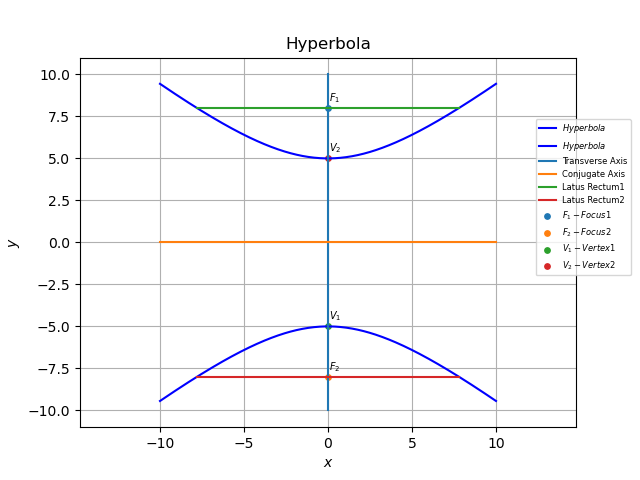
\includegraphics[width=\columnwidth]{chapters/11/11/4/8/figs/hyperbola2}
	\end{center}
\caption{}
\label{fig:chapters/11/11/4/8/Fig1}
\end{figure}


\item Find the equation of the hyperbola that satisfies the conditions - Foci \brak{\pm 4, 0}, the latus rectum is of length 12.
\\
\solution
		\iffalse
\documentclass[journal,12pt,twocolumn]{IEEEtran}
\usepackage{setspace}
\usepackage{gensymb}
\singlespacing
\usepackage[cmex10]{amsmath}
\usepackage{amsthm}
\usepackage{mathrsfs}
\usepackage{txfonts}
\usepackage{stfloats}
\usepackage{bm}
\usepackage{cite}
\usepackage{cases}
\usepackage{subfig}
\usepackage{longtable}
\usepackage{multirow}
\usepackage{enumitem}
\usepackage{mathtools}
\usepackage{steinmetz}
\usepackage{tikz}
\usepackage{circuitikz}
\usepackage{verbatim}
\usepackage{tfrupee}
\usepackage[breaklinks=true]{hyperref}
\usepackage{tkz-euclide}
\usetikzlibrary{calc,math}
\usepackage{listings}
    \usepackage{color}                                            %%
    \usepackage{array}                                            %%
    \usepackage{longtable}                                        %%
    \usepackage{calc}                                             %%
    \usepackage{multirow}                                         %%
    \usepackage{hhline}                                           %%
    \usepackage{ifthen}                                           %%
  %optionally (for landscape tables embedded in another document): %%
    \usepackage{lscape}     
\usepackage{multicol}
\usepackage{chngcntr}
\DeclareMathOperator*{\Res}{Res}
\renewcommand\thesection{\arabic{section}}
\renewcommand\thesubsection{\thesection.\arabic{subsection}}
\renewcommand\thesubsubsection{\thesubsection.\arabic{subsubsection}}

\renewcommand\thesectiondis{\arabic{section}}
\renewcommand\thesubsectiondis{\thesectiondis.\arabic{subsection}}
\renewcommand\thesubsubsectiondis{\thesubsectiondis.\arabic{subsubsection}}

% correct bad hyphenation here
\hyphenation{op-tical net-works semi-conduc-tor}
\def\inputGnumericTable{}                                 %%

\lstset{
frame=single, 
breaklines=true,
columns=fullflexible
}

\begin{document}


\newtheorem{theorem}{Theorem}[section]
\newtheorem{problem}{Problem}
\newtheorem{proposition}{Proposition}[section]
\newtheorem{lemma}{Lemma}[section]
\newtheorem{corollary}[theorem]{Corollary}
\newtheorem{example}{Example}[section]
\newtheorem{definition}[problem]{Definition}
\newcommand{\BEQA}{\begin{eqnarray}}
\newcommand{\EEQA}{\end{eqnarray}}
\newcommand{\define}{\stackrel{\triangle}{=}}

\bibliographystyle{IEEEtran}
\providecommand{\mbf}{\mathbf}
\providecommand{\pr}[1]{\ensuremath{\Pr\left(#1\right)}}
\providecommand{\qfunc}[1]{\ensuremath{Q\left(#1\right)}}
\providecommand{\sbrak}[1]{\ensuremath{{}\left[#1\right]}}
\providecommand{\lsbrak}[1]{\ensuremath{{}\left[#1\right.}}
\providecommand{\rsbrak}[1]{\ensuremath{{}\left.#1\right]}}
\providecommand{\brak}[1]{\ensuremath{\left(#1\right)}}
\providecommand{\lbrak}[1]{\ensuremath{\left(#1\right.}}
\providecommand{\rbrak}[1]{\ensuremath{\left.#1\right)}}
\providecommand{\cbrak}[1]{\ensuremath{\left\{#1\right\}}}
\providecommand{\lcbrak}[1]{\ensuremath{\left\{#1\right.}}
\providecommand{\rcbrak}[1]{\ensuremath{\left.#1\right\}}}
\theoremstyle{remark}
\newtheorem{rem}{Remark}
\newcommand{\sgn}{\mathop{\mathrm{sgn}}}
\providecommand{\abs}[1]{\left\vert#1\right\vert}
\providecommand{\res}[1]{\Res\displaylimits_{#1}} 
\providecommand{\norm}[1]{\left\lVert#1\right\rVert}
\providecommand{\mtx}[1]{\mathbf{#1}}
\providecommand{\mean}[1]{E\left[ #1 \right]}
\providecommand{\fourier}{\overset{\mathcal{F}}{ \rightleftharpoons}}
\providecommand{\system}{\overset{\mathcal{H}}{ \longleftrightarrow}}
\newcommand{\solution}{\noindent \textbf{Solution: }}
\newcommand{\cosec}{\,\text{cosec}\,}
\providecommand{\dec}[2]{\ensuremath{\overset{#1}{\underset{#2}{\gtrless}}}}
\newcommand{\myvec}[1]{\ensuremath{\begin{pmatrix}#1\end{pmatrix}}}
\newcommand{\mydet}[1]{\ensuremath{\begin{vmatrix}#1\end{vmatrix}}}
\numberwithin{equation}{subsection}
\makeatletter
\@addtoreset{figure}{problem}
\makeatother

\let\StandardTheFigure\thefigure
\let\vec\mathbf
\renewcommand{\thefigure}{\theproblem}



\def\putbox#1#2#3{\makebox[0in][l]{\makebox[#1][l]{}\raisebox{\baselineskip}[0in][0in]{\raisebox{#2}[0in][0in]{#3}}}}
     \def\rightbox#1{\makebox[0in][r]{#1}}
     \def\centbox#1{\makebox[0in]{#1}}
     \def\topbox#1{\raisebox{-\baselineskip}[0in][0in]{#1}}
     \def\midbox#1{\raisebox{-0.5\baselineskip}[0in][0in]{#1}}

\vspace{3cm}


\title{Assignment 1}
\author{Jaswanth Chowdary Madala}





% make the title area
\maketitle

\newpage

%\tableofcontents

\bigskip

\renewcommand{\thefigure}{\theenumi}
\renewcommand{\thetable}{\theenumi}


\begin{enumerate}
%\begin{figure}[ht]
%\centering
%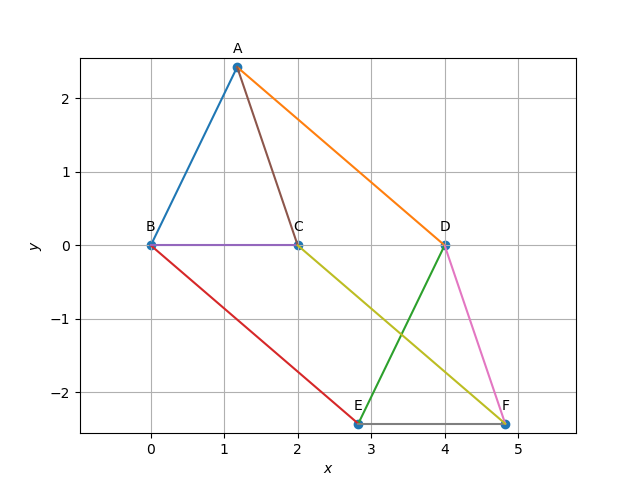
\includegraphics[width = \columnwidth]{"./chapters/11/11/4/13/figs/fig.png"}
%\caption{Graph}
%\label{fig:chapters/11/11/4/13/1}
%\end{figure}

\textbf{Solution:}
\fi
The equation of the conic with focus $\vec{F}$, directrix $\vec{n}^\top\vec{x} = c$ and eccentricity $e$ is given by
\begin{align}
\vec{x}^\top\vec{V}\vec{x} + 2\vec{u}^\top\vec{x} + f = 0
\label{eq:chapters/11/11/4/13/1}
\end{align}
where
\begin{align}
\vec{V} &\triangleq \norm{\vec{n}}^2\vec{I} - e^2\vec{n}\vec{n}^\top \label{eq:chapters/11/11/4/13/2} \\
\vec{u} &\triangleq ce^2\vec{n} - \norm{\vec{n}}^2\vec{F} \label{eq:chapters/11/11/4/13/3} \\
f &\triangleq \norm{\vec{n}}^2\norm{\vec{F}}^2 - c^2e^2 \label{eq:chapters/11/11/4/13/4}
\end{align}
also
\begin{align}
f_0 &= \vec{u}^\top\vec{V}^{-1}\vec{u} - f\\
l &= 2\frac{\sqrt{\abs{f_0\lambda_2}}}{\lambda_1}
\end{align}

\begin{enumerate}
\item $\vec{n}$: Given that the conic has foci as
\begin{align}
\vec{F_1} &= \myvec{4\\0}\\
\vec{F_2} &= \myvec{-4\\0}
\end{align}
The direction vector of $F_1F_2$ is given by
\begin{align}
\vec{m} &= \vec{F_1} - \vec{F_2}\\
&= \myvec{1\\0}
\end{align}
Hence the normal to the directrix is given by,
\begin{align}
\vec{n} = \myvec{1\\0}
\end{align}

\item $\vec{u}$: The centre of the conic is given by
\begin{align}
\vec{c} &= \frac{\vec{F_1} + \vec{F_2}}{2}
\end{align}
\begin{align}
\vec{c} &= \myvec{0\\0}\\
\vec{c} &= -\vec{V}^{-1}\vec{u}
\label{eq:chapters/11/11/4/13/5}
\end{align}
Since $\vec{c} = \vec{0}$ and $\vec{V}^{-1} \neq \vec{0}$, it follows from \eqref{eq:chapters/11/11/4/13/5} that 
\begin{align}
\vec{u} = \myvec{0\\0}
\end{align}

From the above expressions we get
\begin{align}
\vec{V} &= \myvec{1-e^2&0\\0&1} \label{eq:chapters/11/11/4/13/6} \\
\vec{F} &= \myvec{ce^2\\0} \label{eq:chapters/11/11/4/13/7}\\
f &= c^2e^2\brak{e^2-1} \label{eq:chapters/11/11/4/13/8}\\
f_0 &= - f \label{eq:chapters/11/11/4/13/9}\\
l &= 2\frac{\sqrt{\abs{f\lambda_2}}}{\lambda_1}\label{eq:chapters/11/11/4/13/10}
\end{align}

From equation \eqref{eq:chapters/11/11/4/13/6} the eigen values of matrix $\vec{V}$ - $\lambda_1, \lambda_2$ are given by,
\begin{align}
\lambda_1 &= 1-e^2
\label{eq:chapters/11/11/4/13/11}\\
\lambda_2 &= 1
\label{eq:chapters/11/11/4/13/12}
\end{align}

From equation \eqref{eq:chapters/11/11/4/13/7} we get,
\begin{align}
ce^2 = 4 \label{eq:chapters/11/11/4/13/13}
\end{align}
\item Eccentricity: Given that the conic has the latus rectum length 12. Substituting the expressions of $\lambda_1,\lambda_2$ from the equations \eqref{eq:chapters/11/11/4/13/11}, \eqref{eq:chapters/11/11/4/13/12} in \eqref{eq:chapters/11/11/4/13/10} gives
\begin{align}
l = \frac{2ce}{\sqrt{e^2-1}} &= 12\\
\frac{ce}{\sqrt{e^2-1}} &= 6
\end{align}
Substitute the expression of $c$ from \eqref{eq:chapters/11/11/4/13/13} gives,
\begin{align}
\frac{4}{e\sqrt{e^2-1}} &= 6
\end{align}
Squaring on both sides gives,
\begin{align}
9e^2\brak{e^2-1} &= 4\\
9e^4-9e^2-4 &= 0
\label{eq:chapters/11/11/4/13/14}
\end{align}
The equation \eqref{eq:chapters/11/11/4/13/14} is a quadratic equation in $e^2$.
Solving it gives two roots one of which is negative, as $e^2$ is positive we have
\begin{align}
%e^2 &= \frac{-\brak{-9}\pm\sqrt{\brak{-9}^2-4\times9\times\brak{-4}}}{2\times9}\\
e^2 &= \frac{4}{3}
\end{align}
From equation \eqref{eq:chapters/11/11/4/13/8}, \eqref{eq:chapters/11/11/4/13/13}, we get
\begin{align}
f = 4
\end{align} 
\end{enumerate}
The equation of the conic is given by
\begin{align}
\vec{x}^\top\myvec{-\frac{1}{3}&0\\0&1}\vec{x} +4 = 0
\end{align}
\begin{figure}[ht]
\centering
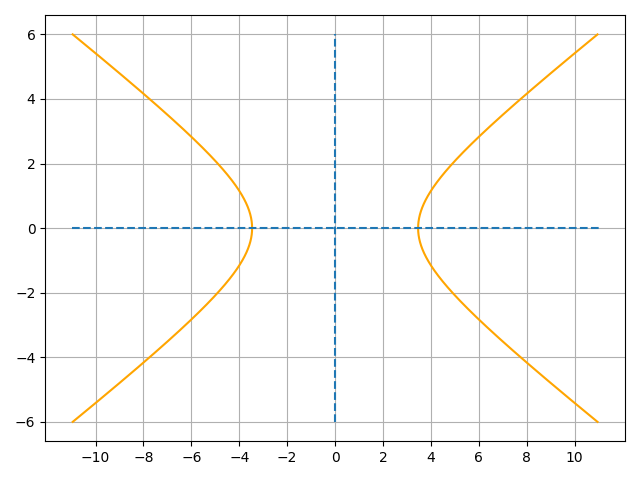
\includegraphics[width = \columnwidth]{chapters/11/11/4/13/figs/fig1.png}
\caption{Graph}
\label{fig:chapters/11/11/4/13/1}
\end{figure}
\begin{table}[h]
\centering
%%%%%%%%%%%%%%%%%%%%%%%%%%%%%%%%%%%%%%%%%%%%%%%%%%%%%%%%%%%%%%%%%%%%%%
%%                                                                  %%
%%  This is a LaTeX2e table fragment exported from Gnumeric.        %%
%%                                                                  %%
%%%%%%%%%%%%%%%%%%%%%%%%%%%%%%%%%%%%%%%%%%%%%%%%%%%%%%%%%%%%%%%%%%%%%%

\begin{center}
\begin{tabular}{|c|c|c|}
\hline
\textbf{Parameter}& \textbf{Description} &\textbf{Value}\\ \hline
$\vec{F_1}$		 &	Focus 1 of hyperbola&$\myvec{4\\0}$\\ \hline
$\vec{F_2}$		 &	Focus 2 of hyperbola&$\myvec{-4\\0}$\\ \hline
$l$		 &  Length of latus rectum&12 \\ \hline
\end{tabular}
\end{center}

\caption{}
\label{tab:chapters/11/11/4/13/1}
\end{table}

    \item Find the equation of the hyperbola whose eccentricity is $e = \frac{4}{3}$
    and whose vertices are
    \begin{align}
        \vec{P_1} = \myvec{7\\0},\ \vec{P_2} = \myvec{-7\\0}
        \label{eq:chapters/11/11/4/14/vert}
    \end{align}
\\
\solution
		\iffalse
\documentclass[journal,12pt,twocolumn]{IEEEtran}
\usepackage{setspace}
\usepackage{gensymb}
\usepackage{xcolor}
\usepackage{caption}
\singlespacing
\usepackage{siunitx}
\usepackage[cmex10]{amsmath}
\usepackage{mathtools}
\usepackage{hyperref}
\usepackage{amsthm}
\usepackage{mathrsfs}
\usepackage{txfonts}
\usepackage{stfloats}
\usepackage{cite}
\usepackage{cases}
\usepackage{subfig}
\usepackage{longtable}
\usepackage{multirow}
\usepackage{enumitem}
\usepackage{bm}
\usepackage{mathtools}
\usepackage{listings}
\usepackage{tikz}
\usetikzlibrary{shapes,arrows,positioning}
\usepackage{circuitikz}
\renewcommand{\vec}[1]{\boldsymbol{\mathbf{#1}}}
\DeclareMathOperator*{\Res}{Res}
\renewcommand\thesection{\arabic{section}}
\renewcommand\thesubsection{\thesection.\arabic{subsection}}
\renewcommand\thesubsubsection{\thesubsection.\arabic{subsubsection}}

\renewcommand\thesectiondis{\arabic{section}}
\renewcommand\thesubsectiondis{\thesectiondis.\arabic{subsection}}
\renewcommand\thesubsubsectiondis{\thesubsectiondis.\arabic{subsubsection}}
\hyphenation{op-tical net-works semi-conduc-tor}

\lstset{
language=Python,
frame=single, 
breaklines=true,
columns=fullflexible
}
\begin{document}
\theoremstyle{definition}
\newtheorem{theorem}{Theorem}[section]
\newtheorem{problem}{Problem}
\newtheorem{proposition}{Proposition}[section]
\newtheorem{lemma}{Lemma}[section]
\newtheorem{corollary}[theorem]{Corollary}
\newtheorem{example}{Example}[section]
\newtheorem{definition}{Definition}[section]
\newcommand{\BEQA}{\begin{eqnarray}}
\newcommand{\EEQA}{\end{eqnarray}}
\newcommand{\define}{\stackrel{\triangle}{=}}
\newcommand{\myvec}[1]{\ensuremath{\begin{pmatrix}#1\end{pmatrix}}}
\newcommand{\mydet}[1]{\ensuremath{\begin{vmatrix}#1\end{vmatrix}}}
\bibliographystyle{IEEEtran}
\providecommand{\nCr}[2]{\,^{#1}C_{#2}} % nCr
\providecommand{\nPr}[2]{\,^{#1}P_{#2}} % nPr
\providecommand{\mbf}{\mathbf}
\providecommand{\pr}[1]{\ensuremath{\Pr\left(#1\right)}}
\providecommand{\qfunc}[1]{\ensuremath{Q\left(#1\right)}}
\providecommand{\sbrak}[1]{\ensuremath{{}\left[#1\right]}}
\providecommand{\lsbrak}[1]{\ensuremath{{}\left[#1\right.}}
\providecommand{\rsbrak}[1]{\ensuremath{{}\left.#1\right]}}
\providecommand{\brak}[1]{\ensuremath{\left(#1\right)}}
\providecommand{\lbrak}[1]{\ensuremath{\left(#1\right.}}
\providecommand{\rbrak}[1]{\ensuremath{\left.#1\right)}}
\providecommand{\cbrak}[1]{\ensuremath{\left\{#1\right\}}}
\providecommand{\lcbrak}[1]{\ensuremath{\left\{#1\right.}}
\providecommand{\rcbrak}[1]{\ensuremath{\left.#1\right\}}}
\theoremstyle{remark}
\newtheorem{rem}{Remark}
\newcommand{\sgn}{\mathop{\mathrm{sgn}}}
\newcommand{\rect}{\mathop{\mathrm{rect}}}
\newcommand{\sinc}{\mathop{\mathrm{sinc}}}
\providecommand{\abs}[1]{\left\vert#1\right\vert}
\providecommand{\res}[1]{\Res\displaylimits_{#1}} 
\providecommand{\norm}[1]{\lVert#1\rVert}
\providecommand{\mtx}[1]{\mathbf{#1}}
\providecommand{\mean}[1]{E\left[ #1 \right]}
\providecommand{\fourier}{\overset{\mathcal{F}}{ \rightleftharpoons}}
\providecommand{\ztrans}{\overset{\mathcal{Z}}{ \rightleftharpoons}}
\providecommand{\system}[1]{\overset{\mathcal{#1}}{ \longleftrightarrow}}
\newcommand{\solution}{\noindent \textbf{Solution: }}
\providecommand{\dec}[2]{\ensuremath{\overset{#1}{\underset{#2}{\gtrless}}}}
\let\StandardTheFigure\thefigure
\def\putbox#1#2#3{\makebox[0in][l]{\makebox[#1][l]{}\raisebox{\baselineskip}[0in][0in]{\raisebox{#2}[0in][0in]{#3}}}}
     \def\rightbox#1{\makebox[0in][r]{#1}}
     \def\centbox#1{\makebox[0in]{#1}}
     \def\topbox#1{\raisebox{-\baselineskip}[0in][0in]{#1}}
     \def\midbox#1{\raisebox{-0.5\baselineskip}[0in][0in]{#1}}

\vspace{3cm}
\title{Conic Assignment}
\author{Gautam Singh}
\maketitle
\bigskip

\begin{abstract}
    This document contains the solution to Question 14 of Exercise 4 in Chapter
    11 of the class 11 NCERT textbook.
\end{abstract}

\begin{enumerate}
\fi
		Let the equation of the conic with focus $\vec{F}$, directrix
    $\vec{n}^\top\vec{x} = c$ and eccentricity $e$ be
    \begin{align}
        \vec{x}^\top\vec{V}\vec{x} + 2\vec{u}^\top\vec{x} + f = 0
        \label{eq:chapters/11/11/4/14/conic-def}
    \end{align}
    where
    \begin{align}
        \vec{V} &\triangleq \norm{\vec{n}}^2\vec{I} - e^2\vec{n}\vec{n}^\top \label{eq:chapters/11/11/4/14/V-def} \\
        \vec{u} &\triangleq ce^2\vec{n} - \norm{\vec{n}}^2\vec{F} \label{eq:chapters/11/11/4/14/u-def} \\
        f &\triangleq \norm{\vec{n}}^2\norm{\vec{F}}^2 - c^2e^2 \label{eq:chapters/11/11/4/14/f-def}
    \end{align}
    The major axis of a conic is the chord which passes through the vertices of the conic.
    The direction vector of the major axis in this case is
    \begin{align}
        \vec{P_2}-\vec{P_1} = \myvec{14\\0}
    \end{align}
    Hence, the normal to the major axis $P_1P_2$ is
    \begin{align}
        \vec{n_M} = \vec{e_2} = \myvec{0\\1}
    \end{align}
    Thus, the equation of the major axis is
    \begin{align}
        \vec{e_2}^\top\vec{x} = \vec{e_2}^\top\myvec{7\\0} = 0
    \end{align}
    which is clearly the $x$-axis.

    Since the conic is a hyperbola whose vertices are given by \eqref{eq:chapters/11/11/4/14/vert}
    and the major axis is the $x$-axis, the directrix is parallel to the $y$-axis.
    Hence,
    \begin{align}
        \vec{n} = \myvec{1\\0}
    \end{align}
    Thus,
    \begin{align}
        \vec{V} = \myvec{1-e^2&0\\0&1} \label{eq:chapters/11/11/4/14/V-val} \\
        \vec{u} = ce^2\myvec{1\\0} - \vec{F} \label{eq:chapters/11/11/4/14/u-val} \\
        f = \norm{\vec{F}}^2 - c^2e^2 \label{eq:chapters/11/11/4/14/f-val}
    \end{align}
    Substituting $\vec{P_1}$ and $\vec{P_2}$ in \eqref{eq:chapters/11/11/4/14/conic-def},
    \begin{align}
        \vec{P_1}^\top\vec{VP_1} + 2\vec{u}^\top\vec{P_1} + f &= 0 \label{eq:chapters/11/11/4/14/ep1} \\
        \vec{P_2}^\top\vec{VP_2} + 2\vec{u}^\top\vec{P_2} + f &= 0 \label{eq:chapters/11/11/4/14/ep2}
    \end{align}
    Subtracting \eqref{eq:chapters/11/11/4/14/ep2} from \eqref{eq:chapters/11/11/4/14/ep1}, and noting that $\vec{P_2} = -\vec{P_1}$,
    \begin{align}
        \vec{u}^\top\vec{P_1} = 0
        \label{eq:chapters/11/11/4/14/u-exp}
    \end{align}
    Hence, from \eqref{eq:chapters/11/11/4/14/vert}, we see that $\vec{u}$ lies on the $y$-axis.
    The general expression of the centre of a conic is given by
    \begin{align}
        \vec{c} &= -\vec{V}^{-1}\vec{u} \\
                &= \frac{1}{e^2-1}\myvec{1&0\\0&1-e^2}\vec{u}
        \label{eq:chapters/11/11/4/14/center}
    \end{align}
    We let $\vec{u} \triangleq \myvec{0\\u}$ and obtain from \eqref{eq:chapters/11/11/4/14/center}
    \begin{align}
        \vec{c} = \myvec{0\\-u} = -\vec{u}
        \label{eq:chapters/11/11/4/14/u-c-0}
    \end{align}
    Since the major axis of the hyperbola is the $x$-axis, we see that $\vec{c}$
    lies on the $x$-axis. Thus, \eqref{eq:chapters/11/11/4/14/u-c-0} implies $\vec{c} = -\vec{u} 
    = \vec{0}$. Thus, from \eqref{eq:chapters/11/11/4/14/u-val},
    \begin{align}
        \vec{F} = \myvec{ce^2\\0}
        \label{eq:chapters/11/11/4/14/F-c-e}
    \end{align}
    and so,
    \begin{align}
        f = c^2e^2\brak{e^2-1}
        \label{eq:chapters/11/11/4/14/f-c-e}
    \end{align}
    Putting $\vec{x} = \vec{P_1}$ or $\vec{x} = \vec{P_2}$ in \eqref{eq:chapters/11/11/4/14/conic-def} 
    and using \eqref{eq:chapters/11/11/4/14/F-c-e} and \eqref{eq:chapters/11/11/4/14/f-c-e},
    \begin{align}
        \myvec{\pm7&0}\myvec{1-e^2&0\\0&1}\myvec{0\\\pm7} + f &= 0 \\
        \implies 49e^2 - f = 49 \label{eq:chapters/11/11/4/14/e1}
    \end{align}
    Since $e = \frac{4}{3}$, \eqref{eq:chapters/11/11/4/14/e1} implies
    \begin{align}
        f = 49\brak{e^2-1} = \frac{343}{9}
    \end{align}
    Therefore, the equation of the conic is
    \begin{align}
        \vec{x}^\top\myvec{-\frac{7}{9}&0\\0&1}\vec{x} + \frac{343}{9} = 0
    \end{align}
    The situation is illustrated in Fig. \ref{fig:chapters/11/11/4/14/hyperbola}.
    \begin{figure}[!ht]
        \centering
        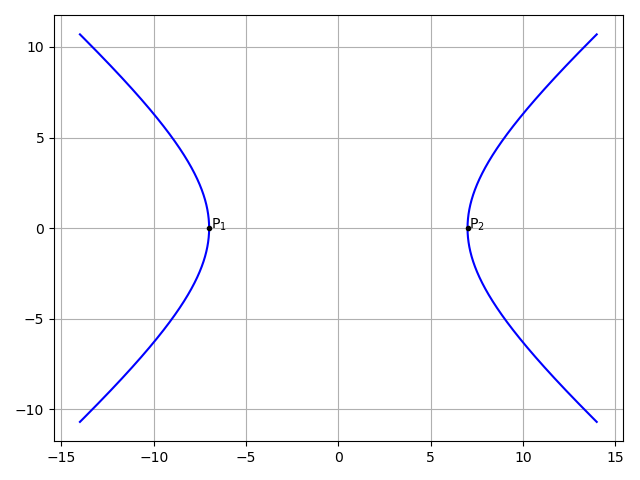
\includegraphics[width=\columnwidth]{chapters/11/11/4/14/figs/hyperbola.png}
        \caption{Locus of the required hyperbola.}
        \label{fig:chapters/11/11/4/14/hyperbola}
    \end{figure}


\end{enumerate}
